\chapter{Le projet Yuukou 2}

\section{Recherches}

\subsection{Architecture du projet}

Le premier travail a \'et\'e la r\'eflexion sur comment mettre en place une solution pouvant communiquer avec Nagios dont une description sera faite en~\ref{section:nagios}.
Les figures~\ref{figure:architectureProjetServiceWeb} et~\ref{figure:architectureProjetAffichage} pr\'esentent le fruit des recherches qui ont \'et\'e faites sur la mise en place du projet \YuukouII.

\begin{figure}[!ht]
	\centering
	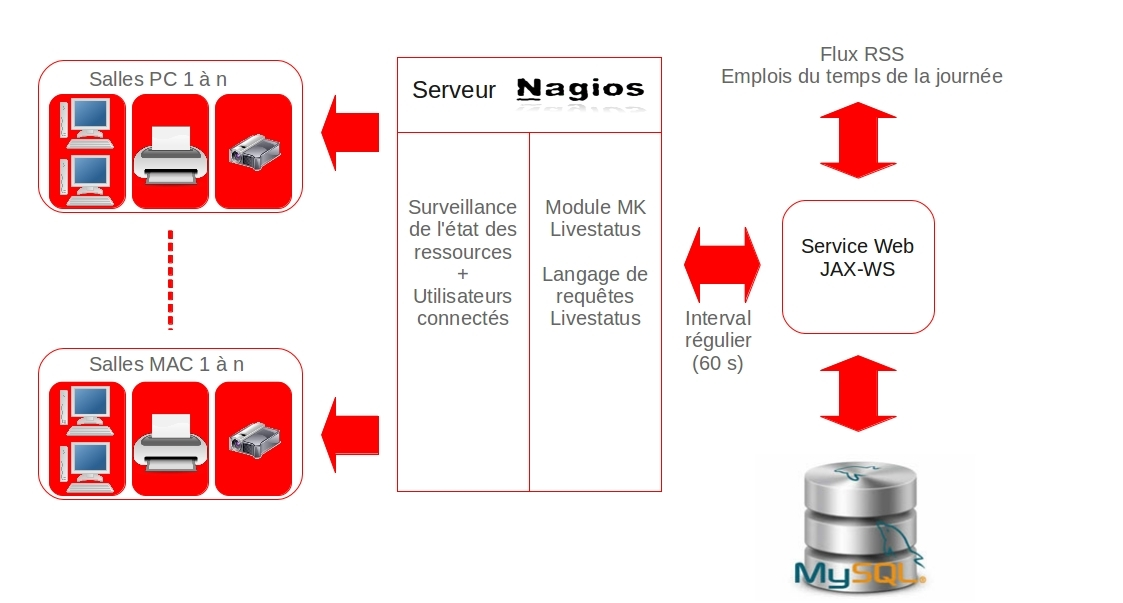
\includegraphics[scale=0.35]{architectureProjetServiceWeb.jpg}
	\caption{Architecture du projet, partie service Web}
	\label{figure:architectureProjetServiceWeb}

\end{figure}

\begin{figure}[!ht]
	\centering
	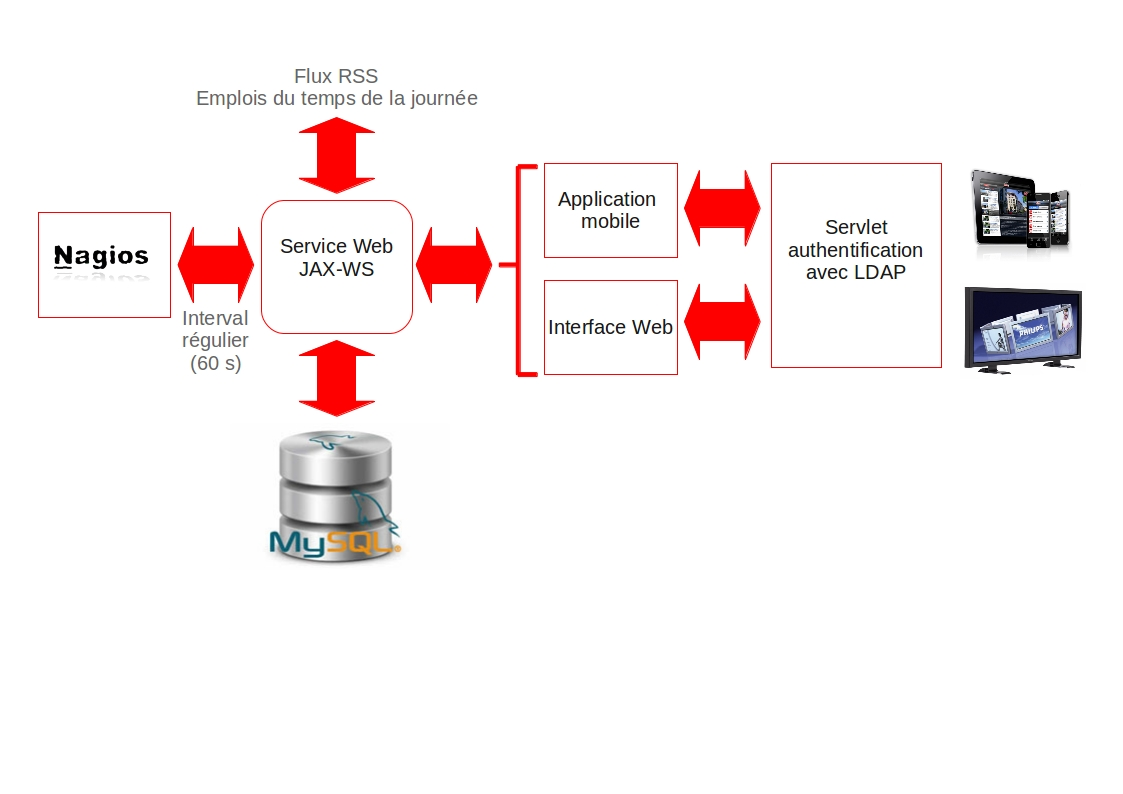
\includegraphics[scale=0.35]{architectureProjetAffichage.jpg}
	\caption{Architecture du projet, partie affichage}
	\label{figure:architectureProjetAffichage}

\end{figure}

\subsubsection{Partie service Web}

Basiquement Nagios sert \`a surveiller les ressources auxquelles il lui est permis d'acc\'eder.
De ce fait, il doit garder des traces des informations qu'il r\'ecup\`ere.
Ces informations sont stock\'ees dans un fichier.
C'est pourquoi un plugin existe sp\'ecialement pour acc\'eder aux informations contenu dans ce fichier. 
Le plugin \textit{MK Livestatus} permet \`a l'aide d'un langage de requ\^etes qui lui est propre, de r\'ecup\'erer les informations que garde Nagios.

Le service Web doit permettre, dans un premier temps, de r\'ecup\'erer toutes les informations utiles pour un archivage des donn\'ees.
Elles sont stock\'ees dans une base de donn\'ees MySQL.
\noindent Ces informations sont :
\begin{itemize}
	\item les donn\'ees r\'ecup\'er\'ees via le plugin \textit{MK Livestatus}, la r\'ecup\'eration doit \^etre faite \`a intervalles r\'eguliers;
	\item les diff\'erents emplois du temps de toutes les salles que Nagios surveille, la r\'ecup\'eration doit \^etre faite une fois par jour;
	\item les donn\'ees sur un utilisateur inconnu (nom, pr\'enom, r\^ole : \'etudiant par exemple, photo) via un serveur LDAP.

\end{itemize}

\subsubsection{Partie affichage}

Dans un deuxi\`eme temps, le service Web doit pouvoir retourner ces informations tri\'ees \`a un utilisateur normal ou un administrateur afin de garantir l'affichage sous la forme d'une application mobile ou d'une interface Web.
La r\'eflexion doit ainsi se porter sur le contenu des diff\'erentes m\'ethodes auxquelles un utilisateur pourra avoir acc\`es (en fonction qu'il soit administrateur ou non).
Le but \'etant un affichage le plus rapide possible des informations demand\'ees.

L'utilisateur doit s'authentifier via un Servlet$^*$ qui communique avec LDAP$^*$ et qui donne un acc\`es \`a l'application.
Le reste de la communication est s\'ecuris\'ee comme expliqu\'e dans le~\ref{section:securisation}.

Le dernier point est le format des donn\'ees qui seront \'echang\'ees entre le service Web et l'application cliente.

\subsection{Nagios}
\label{section:nagios}

\begin{figure}[!ht]
	\centering
	
\includegraphics[scale=0.5]{nagiosLogo.jpg}
	\caption{Logo de Nagios}

\end{figure}

\subsubsection{Pr\'esentation}

Nagios est une application permettant la surveillance syst\`eme et r\'eseau de toute une infrastructure informatique.
Nagios compl\`ete cette surveillance en offrant la possibilit\'e d'alerter les \'equipe en charge de l'infrastructure en cas d'apparition de probl\`emes comme une panne ou encore un fonctionnement anormal.
C'est actuellement la solution de surveillance la plus efficace du march\'e.

\parpic{
	\begin{minipage}{0.20\textwidth}
		
\includegraphics[scale=0.6]{netsaintLogo.jpg}
	\end{minipage}}
Nagios a \'et\'e cr\'e\'e en 1999 et portait initialement le nom de \textit{NetSaint Network Monitor}.
Il est \'ecrit en C et est con\c{c}u pour un environnement Unix.
Le projet a \'et\'e maintenu jusqu'en 2002 avant de changer de nom pour devenir Nagios en r\'eponse \`a une contestation judiciaire par les propri\'etaires d'une marque similaire.
N.A.G.I.O.S. est l'acronyme r\'ecursif de \og{}\textit{Nagios Ain't Gonna Insist On Sainthood}\fg{} o\`u Sainthood est une r\'ef\'erence \`a \textit{NetSaint}.

Maintenant connu sous le nom de Nagios XI, Nagios est un logiciel libre sous la licence GNU GPL V2. Il est disponible sous sa version 2011R2.4 datant du 24 avril 2012.

\subsubsection{Fonctionnement}

\noindent L'architecture de base de Nagios est tr\'es simple, elle comporte :
\begin{itemize}
	\item un ordonnanceur pour g\'erer les v\'erification ainsi que les actions \`a prendre sur les diff\'erents incidents;
	\item une partie graphique : visible \`a travers un simple serveur Web;
	\item des sondes : greffons (ou \textit{plugins} en anglais) dans Nagios, ce sont de petits scripts permettant d'effectuer diverses v\'erifications.

\end{itemize}

Basiquement, Nagios est un moteur d'ordonnancement de v\'erifications diverses et vari\'ees dont les v\'erifications sont effectu\'ees via des greffons.
Ces v\'erifications peuvent \^etre la charge d'utilisation du CPU\protect\footnote{Central Processing Unit ou processeur en fran\c{c}ais}, l'espace disque utilis\'e ou encore qui est connect\'e actuellement.
Dans le cadre de la v\'erification de l'infrastructure, deux types de machines sont observ\'ees : les ordinateurs dot\'es de Windows et les ordinateurs dot\'es de Macintosh.

Nagios \'etant install\'e et fonctionnel depuis un peu plus d'un an sur le site de New Cavendish, les greffons pour observ\'er les deux types de machines ont d\'ej\`a \'et\'e d\'evelopp\'es.
Pour les machines fonctionnant sous Windows, le greffon est en fait l'appel \`a la commande Unix \textit{Winexe} qui permet l'ex\'ecution de commandes \`a distance sur des machines Windows.
Pour les machines fonctionnant sous Macintosh, le greffon effectue une connexion SSH\protect\footnote{SecureShell}, offrant une connexion s\'ecuris\'ee sur une machine distante pour ensuite ex\'ecuter la commande Unix \textit{who} permettant l'obtention de l'utilisateur connect\'e.

\subsubsection{\og{}Monitoring\fg{} \`a l'universit\'e}

Initialement, Nagios surveillait juste les machines se situant sur le campus de New Cavendish, soit 31 salles PC seulement machines.
Actuellement, ce sont 102 salles qui sont sous la surveillance de Nagios, soit 99 salles utilisant Windows soit 1920 PC, 3 salles utilisant des Macintosh soit 63 MAC, pour un total de 1983 machines \`a travers toute l'universit\'e.
Il faut not\'e que seuls les Macintosh de New Cavendish sont sous surveillance, les autres n\'ecessitant des acc\`es diff\'erents. TODO VERIFIER
De ce fait, le nombre de machines devrait augmenter par la suite.







TODO winexe execute commande distante 


\subsection{La notion de service Web}
\label{section:serviceWeb}

\subsection{L'API JAX-WS}

\subsection{L'IDE NetBeans}

\subsection{Le serveur Web Glassfish}

\subsection{Le SGBD MySQL}

\subsection{Data Access Object}

\subsection{Le format de retour : JSon}

\section{Communication avec Nagios}

\subsection{Le plugin MK Livestatus}

\subsection{Requ\^etes pour Nagios}

\subsection{R\'ecup\'eration des informations}

\section{Gestion de la base de donn\'ees}

\subsection{Structure de la base de donn\'ees}

\subsection{Explications}

\subsection{G\'en\'eration de la configuration Nagios \`a partir de la base de donn\'ees}

\section{Le service Web}

\subsection{Mise en place}

\subsection{Le cycle principal}

\subsection{Les fonctionnalit\'es publiques}

\subsection{Les fonctionnalit\'es priv\'ees}

\subsection{Le retour des informations}

\subsection{S\'ecurisation du service Web}
\label{section:securisation}

\section{Gestion de l'emploi du temps}

\subsection{Les flux RSS de l'universit\'e}

\subsection{Correspondance des salles}

\section{Tests du service Web}

\subsection{Mise en place d'un client}

\subsection{Consommation les m\'ethodes}

\section{Am\'eliorations possibles}

\section{Probl\`emes rencontr\'es}


\clearpage
